\documentclass{article}
\usepackage[utf8]{inputenc}           % Use uft8 enconding to have a wide
                                      % number of symbols available
\usepackage[spanish]{babel}           % Configure the text language
                                      % to know where to put the hyphen in a 
                                      % line break
\usepackage{graphicx}                 % To include images
\usepackage{anysize}                  % Allows marginsize command
\usepackage{fancyhdr}                 % Configure the header and footer  
\usepackage{titlesec}                 % Changes the section titles properties
\usepackage{amsmath}                  % Active wide number of math symbols
\usepackage{amssymb}                  % Math symbols such as semijoin
\usepackage{longtable}                % Multiple-page table
\usepackage[export]{adjustbox}        % Allows to resize tables
\usepackage{enumitem}                 % Controls the item position 
\usepackage{listings}                 % Package for code fences
%\usepackage{xcolor}                   % Create colors
\usepackage[
  table,
  svgnames,
  dvipsnames
]{xcolor}                             % Colors for code fences and 
                                      %table (rowcolor)
\usepackage{textcomp}                 % Helps to display quotes symbols properly
\usepackage{array}                    % Align fix size columns in tables
\usepackage{multicol}
\usepackage{subcaption}

\decimalpoint%                        % Use dot instead of comma to write 
                                      % decimal numbers
\setlength{\parindent}{0in}           % No indentation at first paragraph

\renewcommand{\familydefault}{\sfdefault} % Changing font
\titleformat*{\section}{\large\bfseries}  % Change section size
\marginsize{1.5cm}{2cm}{1.2cm}{1cm}       % {left}{right}{above}{below}
\setlength{\headsep}{0.3in}               % Changing headsep length
                                          % headsep is the vertical length 
                                          % between header an text area
\lstset{upquote=true}                     % For display quotes and double 
                                          % quoutes in a better style

% Defining column content alignment for fix size columns
\newcolumntype{L}[1]{>{\raggedright\let\newline\\\arraybackslash\hspace{0pt}}m{#1}}
\newcolumntype{C}[1]{>{\centering\let\newline\\\arraybackslash\hspace{0pt}}m{#1}}
\newcolumntype{R}[1]{>{\raggedleft\let\newline\\\arraybackslash\hspace{0pt}}m{#1}}  

%%%%%%%%%%%%%%%%%%%%%%%%%%%%%%%%%%%%%%%%%%%%%%%%%%%%%%%%%%%%%%%%%%%%%%%%%%%%%%%
%%%%%%%%%%                        Code style                         %%%%%%%%%%
%%%%%%%%%%%%%%%%%%%%%%%%%%%%%%%%%%%%%%%%%%%%%%%%%%%%%%%%%%%%%%%%%%%%%%%%%%%%%%%

\definecolor{codegreen}{rgb}{0,0.6,0}
\definecolor{codegray}{rgb}{0.5,0.5,0.5}
\definecolor{codepurple}{rgb}{0.58,0,0.82}
\definecolor{backcolour}{rgb}{1,1,1}

\lstdefinestyle{mystyle}{
  backgroundcolor=\color{backcolour},   
  commentstyle=\color{codegreen},
  keywordstyle=\color{magenta},
  numberstyle=\tiny\color{codegray},
  stringstyle=\color{codepurple},
  %
  basicstyle=\ttfamily\footnotesize,
  captionpos=b,                    
  breakatwhitespace=false,         
  breaklines=true,                 
  keepspaces=true,                 
  showspaces=false,                
  showstringspaces=false,
  showtabs=false,                  
  %
  tabsize=2
  % Diplay number to the left
  % numbers=left,                    
  % numbersep=5pt,                  
}

\lstset{style=mystyle}


%%%%%%%%%%%%%%%%%%%%%%%%%%%%%%%%%%%%%%%%%%%%%%%%%%%%%%%%%%%%%%%%%%%%%%%%%%%%%%%
%%%%%%%%%%                        Header Style                       %%%%%%%%%%
%%%%%%%%%%%%%%%%%%%%%%%%%%%%%%%%%%%%%%%%%%%%%%%%%%%%%%%%%%%%%%%%%%%%%%%%%%%%%%%

\pagestyle{fancy}
\fancyhf{}
\renewcommand{\headrulewidth}{0pt}

% Right header
% The right header has 
%   the subject title,
%   subtitle and 
%   the university logo
\fancyhead[R]{
    \begin{tabular}{l}
        \materia \\ 
        \actividad%
    \end{tabular}
    \,% Adding space between titles and logo    
    \rule[-1.75\baselineskip]{0pt}{0pt}
    % Strut to ensure a 1/4 \baselineskip between image and header rule
    
\includegraphics[height=3\baselineskip,valign=c]{unam}
}

%%%%%%%%%%%%%%%%%%%%%%%%%%%%%%%%%%%%%%%%%%%%%%%%%%%%%%%%%%%%%%%%%%%%%%%%%%%%%%%
%%%%%%%%%%              Cover page generator command                 %%%%%%%%%%
%%%%%%%%%%%%%%%%%%%%%%%%%%%%%%%%%%%%%%%%%%%%%%%%%%%%%%%%%%%%%%%%%%%%%%%%%%%%%%%

\newcommand{\coverPage}{
\thispagestyle{empty}
  \begin{minipage}[t][5cm][t]{0.2\linewidth}
    
\includegraphics[width=2.5cm]{unam.jpg}

    \vspace{10cm}
    % The following space is mandatory to display correct layout

    
\includegraphics[width=2.5cm]{fiblack}
  \end{minipage}
  %
  \begin{minipage}[t]{0.7\linewidth}
    \vspace{-2.5cm}
    \LARGE{\textbf{\university}}\\
    \Large{\textbf{\faculty}} \\
  
    \large{\semestre}\\[2cm]
  
    \large{\textbf{\materia (\clave)}}\\
    \large{\textbf{Gpo: \grupo}}\\[5mm]
    \large{\textbf{Profesor:} \profesor}\\ [1.5cm]
    \begin{center}
        \LARGE{\textbf{\actividad}}\\
        \LARGE{\textbf{\titulo}}\\
    \end{center}
  
    \vspace{3.3cm}
  
    \large{\textbf{Alumno:} \alumno} \\[1.5cm]
    %\large{
    %  \begin{itemize}[ noitemsep, align=left ]
    %    \item [\textbf{Alumno(s):}] 
    %      \begin{flushright}
    %        \alumno
    %      \end{flushright}
    %  \end{itemize}
    %} \vspace{1.5cm}
  
    \begin{flushright}
        \fechaEntrega%
    \end{flushright}
  \end{minipage}

\newpage
}

\begin{document}

%%%%%%%%%%%%%%%%%%%%%%%%%%%%%%%%%%%%%%%%%%%%%%%%%%%%%%%%%%%%%%%%%%%%%%%%%%%%%%%
%%%%%%%%%%                Variables definition                       %%%%%%%%%%
%%%%%%%%%%%%%%%%%%%%%%%%%%%%%%%%%%%%%%%%%%%%%%%%%%%%%%%%%%%%%%%%%%%%%%%%%%%%%%%

\newcommand{\university}{Universidad Nacional Autónoma de México}
\newcommand{\faculty}{Facultad de Ingeniería}
\newcommand{\semestre}{2021-1}
\newcommand{\materia}{BDA}
\newcommand{\clave}{2929}
\newcommand{\grupo}{1}
\newcommand{\profesor}{Ing. Rodriguez Campos \textsc{Jorge Alberto}}

\newcommand{\alumno}{Francisco Pablo \textsc{Rodrigo}}
\newcommand{\actividad}{Tema 04 \\ Ejercicio práctico 04}
\newcommand{\titulo}{Administración de las estructuras de memoria}

\newcommand{\fechaEntrega}{01 de enero de 2021}

\newcommand{\codedir}{tema04-ej-prac-04-codigo}
\graphicspath{{assets/}{tema04-ej-prac-04.assets/}}

\coverPage%


%%%%%%%%%%%%%%%%%%%%%%%%%%%%%%%%%%%%%%%%%%%%%%%%%%%%%%%%%%%%%%%%%%%%%%%%%%%%%%%
%%%%%%%%%%                        Contents                           %%%%%%%%%%
%%%%%%%%%%%%%%%%%%%%%%%%%%%%%%%%%%%%%%%%%%%%%%%%%%%%%%%%%%%%%%%%%%%%%%%%%%%%%%%

\section*{Objetivo}

Comprender y poner en práctica el cálculo y las configuraciones de los
parámetros de una base de datos para modificar los modos de administración de la
memoria: automática, automática compartida y manual.

\section*{C1}

\subsection*{El código del script \texttt{s-01-objetos-iniciales.sql}}

\lstinputlisting[language=SQL]{\codedir/s-01-objetos-iniciales.sql}

\subsection*{La evidencia que muestra la ejecución del procedimiento}

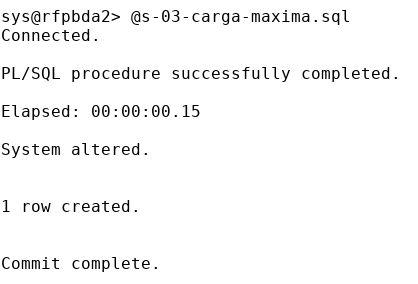
\includegraphics[width=0.4\linewidth]{c1}

\subsection*{Respuestas de las preguntas A, B, C y D}

\begin{enumerate}[label=\Alph*.]
  \item ¿Cuánto tiempo tardó en ejecutar el procedimiento que simula una 
    carga máxima? \\[3mm]
    0.15 segundos

  \item ¿Por qué razón los valores de los parámetros en 
    \texttt{t02\_memory\_param\_values} es cero parámetros es cero, y en la 
    tabla \texttt{t01\_memory\_areas}, la memoria asignada es mayor a cero?
    \\[3mm]
    Los parámetros de la tabla 2 indican el tipo de administración de memoria,
    por ejemplo, si esta configurado en modo automático o manual. Los valores
    son configurados por el DBA. Sin embargo, en la primera tabla, se indica el
    valor reservado de cada estructura de memoria, sin importar el tipo de
    administración que se encuentre configurado.

  \item Considerar los datos de la tabla \texttt{t01\_memory\_areas} con 
    id = 2. Calcular la cantidad de memoria de la SGA que está actualmente 
    en uso ( es decir, no considerar la memoria libre de la SGA)\\[3mm]
    767 - 364 = 403 M

  \item Considerar el valor de la última columna de la tabla 
    \texttt{t01\_memory\_areas} con id = 2. Este valor fue calculado por la 
    instancia y corresponde al valor recomendado de memoria para ser asignado 
    a la PGA en una BD tradicional. ¿Qué porcentaje del total de la SGA le 
    corresponde a este valor? \\[3mm]
    Aproximadamente el 47\%
  \item Describir las diferencias encontradas en los 3 registros de 
    Si se deseara \texttt{t01\_memory\_areas} realizar una configuración 
    manual de la memoria máxima para ser asignada a la PGA, con base a los 
    valores de estos 3 registros, ¿Qué valor tendría esta configuración manual?
    \\[4mm]
    Algunas columnas tienen los mismos valores en los 3 registros, otras como 
    \texttt{buffer cache size}, \texttt{shared pool size}, \texttt{large pool
    size} y \texttt{max pga allocated} tienen valores distintos. De acuerdo a lo
    que hemos aprendido, los parámetros que variaron se debido a que se realizó
    una consulta la cual que hizo que varios grupos de registros se cargaran a
    memoria. El área con mayor carga debió ser la relacionada con la PGA.
\end{enumerate}

\section*{C2}

\subsection*{El contenido del script \texttt{s-04-automatic-shared.sql}}

\lstinputlisting[language=SQL]{\codedir/s-04-automatic-shared.sql}

\subsection*{Respuestas de las preguntas A, B, C y D}

\begin{enumerate}[label=\Alph*.]
  \item ¿Cuál fue el valor obtenido al ejecutar la fórmula anterior?\\[4mm]
  pga\_aggregate\_target debe ser igual a 363M
  \item ¿Para qué se utilizó el valor obtenido al evaluar la fórmula?\\[4mm]
    En este ejercicio se tenía que considerar los valores de
    \texttt{max\_pga\_allocated} para determinar el valor manual de la SGA. Sin
    embargo, \textbf{la primera vez que realicé el ejercicio} obtuve un valor de
    363M en el primer registro. Esto se debio a que previamente había estresado
    a la PGA con las creación de todas las tablas de la práctica.
    Tomé ese valor debido a que fue el más alto. Lo que se esperaba es que el
    valor último fuera el más alto. 
    Otro punto a considerar fue el hecho de que la memoria utilizada por la SGA
    fue de 413M, por lo que si se sumaba el valor de la PGA con este valor se
    obtendría algo similiar a 767 M.
  \item ¿Cuánta memoria libre tiene la SGA?\\[4mm]
    Fue de 404M
  \item Calcular la diferencia entre la memoria libre de la SGA y el valor 
    máximo de memoria PGA que se obtuvo al ejecutar el script 
    \texttt{s-03-carga-maxima.sql}. ¿Qué interpretación o significado representa 
    esta diferencia? \\[4mm]
    \textbf{Tomando los valores de la ejecución más reciente} \\
    364 - 106.43 = 257.57
    Indica que aún existe la posiblidad de que nuestra PGA pueda tomar un valor 
    mayor que el que indica el registro de carga máxima.
\end{enumerate}
\section*{C3. Contenido del script \texttt{s-05-manual-shared.sql}}

\lstinputlisting[language=SQL]{\codedir/s-05-manual-shared.sql}

\section*{C4}

\subsection*{El contenido del script \texttt{s-06-automatic-memory.sql} }

\lstinputlisting[language=SQL]{\codedir/s-06-automatic-memory.sql}

\subsection*{El contenido de las 3 tablas creadas}

\textbf{NOTA: Se incluye la captura de pantalla de la ejecución más reciente. En
ejecuciones anteriores se había obtenido valores mayores para
\texttt{max\_pga\_allocated}, sin embargo, se sobreescribiendo en ejecuciones
posteriores }\\

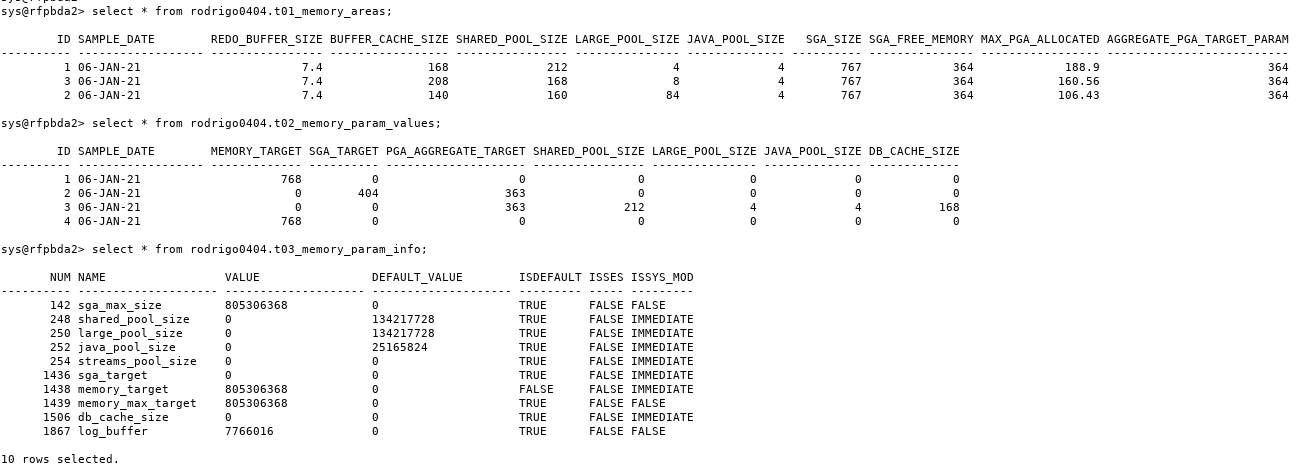
\includegraphics[width=\linewidth]{c4}

\section*{C5. Validador}

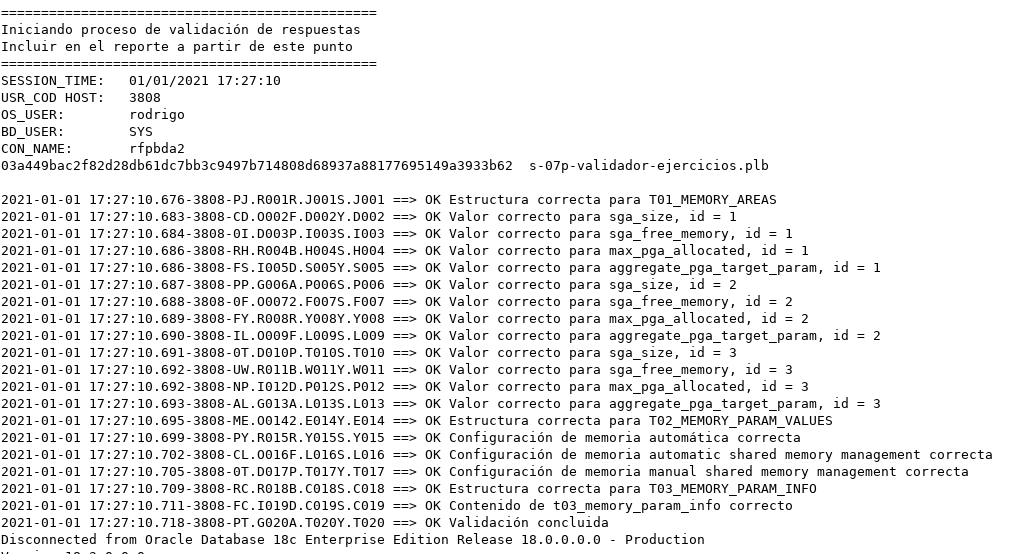
\includegraphics[width=\linewidth]{bda-t04-ep04-validador}

\section*{Comentarios y conclusiones}

Al inicio de este ejercicio no tenía en cuenta la diferencia entre los valores
mostrados por el comando \texttt{show parameter} y por las vista que contiene
los datos de los valores de las estructuras de memoria. Afortunamente este
ejercicio me hizo aprender la diferencia entre cada uno.\\

Por otra parte, se reconoció la importancia de tener configurado correctamente
los parámetros para la administración de la memoria de la base de datos. Uno
solo parámetro configurado de manera errónea podría desencadenar que otros
parámetros se configuren de manera incorrecta, lo cual se traduce en un
degradamiento del rendimiento de nuestra base de datos.

\begin{thebibliography}{99}
    \bibitem{burleson} Burleson Consulting. \textit{Oracle tips } en 
    \texttt{http://www.dba-oracle.com/oracle\_news/}
  \bibitem{oracle} Oracle Help Center. \textit{Database Performance Tuning 
    Guide} en \texttt{https://docs.oracle.com/database/\\%
    121/TGDBA/tune\_buffer\_cache.htm\#TGDBA294}
\end{thebibliography}

\end{document}
